Durante esta seção será abordado o método de funcionamento da luva Hand.io que se propõe a responder os problemas de pesquisa que foram levantados 

\section{Método de Execução da Hand.io}



A luva Hand.io é um dispositivo vestível que conta com um acelerômetro e um giroscópio integrados, a comunicação entre o usuário e os dispositivos eletro-eletrônicos é realizada através de uma central de processamento de padrões e execução de ações tendo a conexão realizada entre os dois através de uma conexão sem fio utilizando o protocolo de IEEE 802.11 \cite{802.11:1997}


\todo{Apresentar um descrição da visão geral do método proposto usando a big picture}

%\begin{figure}
%	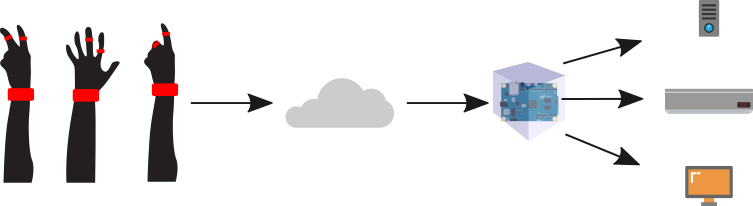
\includegraphics{big_picture}
%\end{figure}






\section{Captura de Dados Baseado em Movimentos da 
Amplitude de Punho e Mão}

Durante o funcionamento normal da luva hand.io o usuário irá 

\section{Reconhecimento de Padrões Baseado em Movimentos e Ações}

O processamento e o reconhecimento dos gestos realizados pelo usuário são processados por um computador localizado na central de processamento e controle

\section{Modelo de Conexão Entre Dispositivos Eletrônicos}

\section{Inferência de Comportamentos para Acionamento de Dispositivos Eletrotônicos}

\section{Modelo de Prototipação}

\begin{figure}
    \centering
    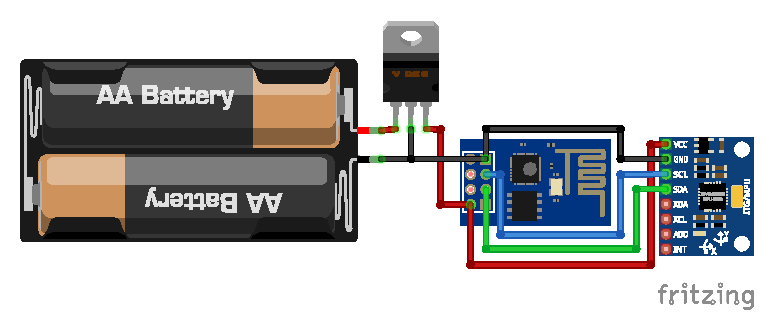
\includegraphics{resources/esquematico_tcc_bb.pdf}
    \caption{Esquemático do protótipo da luva}
    \label{fig:my_label}
\end{figure}

\begin{figure}
    \centering
    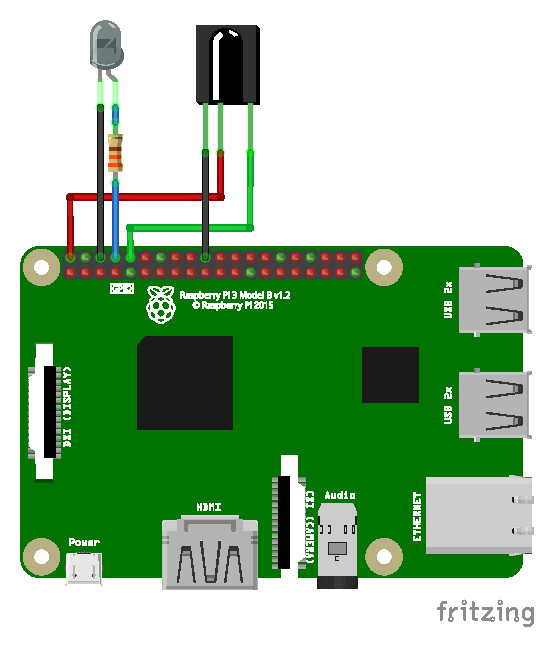
\includegraphics{resources/esquematico_central_bb.pdf}
    \caption{Esquematico da central de processamento de sinais e execução de ações}
    \label{fig:esq_central}
\end{figure}

%\section{Cronograma}